\headline{{\textbf{\Large\sffamily A Bonsai Journey Across Borders:}}\\
          {\textbf{\large\sffamily Mark Angold Shares Lessons from Europe}}}
\label{2025-05-marktalk}
\noindent
% At our recent Twickenham Bonsai Club meeting, we were treated to a rich and insightful presentation by Mark Angold, founder of Shinka Bonsai. In just under an hour, Mark managed to distil years of learning and hands\--on experience into an engaging journey through the bonsai landscapes of Europe and beyond.

% Mark's presentation was refreshingly practical. As he passed around photographs of trees he's worked on with artists across the continent, each image became a window into both technique and philosophy. From Mauro Stemberger's dramatic stylings to Gabriel Romero's refined repotting and Rafael Torres' disciplined root care, every tree had a story --- and a lesson.

At our recent Twickenham Bonsai Club meeting, Mark Angold, founder of Shinka Bonsai, gave a rich and engaging presentation. In under an hour, he shared years of experience, guiding us through bonsai practices across Europe.

Mark's talk was practical and hands\--on. Passing around photos of trees he's worked on with various artists, each image highlighted a key technique or philosophy. From Mauro Stemberger's dramatic styling to Gabriel Romero's refined repotting and Rafael Torres' focus on roots, every tree shared a story --- and a lesson.

\medskip
\topic{Roots First: Working with Gabriel Romero}
\noindent
One of Mark's key influences is Gabriel Romero from Spain, with whom he worked during a visit to the UK. Though Gabriel speaks little English, their connection was immediate --- a shared language spoken through trees. \textit{``We were basically holding two conversations at once,''} Mark recalled, \textit{``one verbal, one with our hands in the soil.''}

Gabriel's approach is bold. He bare\--rooted and repotted two Sabina junipers --- high\--risk procedures that paid off. His method? Hose off all old soil, reset fully after collection, and prioritise strong root work early on. He uses a 50/50 mix of akadama and pumice and waters heavily, sometimes multiple times a day in heat. Sabinas, he noted, handle moisture well.

Photos of the Sabinas before and after showed just how well this approach can work. \textit{``If you get the roots right,''} Gabriel told Mark, ``the tree will do the rest.'' % That philosophy stuck.

\medskip
\topic{Post\--Repot Recovery: Rafael Torres' Pine Protocol}
\noindent
In Spain, Mark spent time with Rafael Torres, known for his remarkable collected material --- wild olives, ancient junipers, and mature pines. What surprised Mark most was Rafael's approach to repotting: even black pines, typically handled conservatively, were completely bare\--rooted on arrival.

Key to this strategy is the recovery environment. Rafael places all newly repotted trees in a greenhouse or poly tunnel, maintaining high humidity and moderate warmth (15--30°C). Watering is minimal --- humidity triggers root growth while reducing rot risk. \textit{``The difference was striking,''} Mark said. \textit{``Pines inside grew two or three inches while the outdoor ones hadn't moved.''}

This controlled recovery environment was a major takeaway: it's not just about how you repot, but how you manage the weeks that follow.

\medskip
\topic{Deadwood and Detail: A Workshop in Caz's Garden}
\noindent
Back in the UK, Mark joined Caroline Scott --- or Caz --- for a workshop in her garden, alongside Portuguese artist Andrés Bicocca. The focus was carving: preserving and enhancing natural movement in deadwood. Caz's approach is traditional --- hammer and chisel first, to reveal natural grain and structure, followed by selective sandblasting.

Mark was especially impressed by the realism this method achieved. \textit{``With power tools, you can destroy the natural texture. But with this approach, you're revealing what's already there --- you're not imposing anything.''}
%
Caz uses rounded grit for sandblasting, which cleans without damaging hardwood. While sandblasting gear is accessible in the UK, good blasting media isn't --- she sources hers from contacts in Belgium.

The day offered a broader reflection on artistry: it's about restraint and observation. Let the tree emerge; don't force it.

\medskip
\topic{Local Lessons: Soil, Substrate, and Shared Learning}
\noindent
Mark also reflected on work closer to home. During a recent repotting session with Michael Cheong, he encountered a struggling maple in poor\--quality soil --- mostly brick dust from a commercial mix. The roots were weak and water retention inconsistent.

After repotting into a mix of akadama and pumice, the tree began to recover. The message was clear: avoid materials like brick, cat litter, or John Innes-based soils. \textit{``They just don't drain well or hold structure over time,''} Mark warned. \textit{``Good soil isn't cheap, but over five or six years, it pays for itself in tree health.''}

Soil choice, he emphasised, must suit both the species and your environment. \textit{``Use the right soil for the right tree --- and for where you live.''}

\medskip
\topic{Beginnings, Influence, and Evolution}
\noindent
Mark's bonsai journey began in 2020 with a humble Chinese elm gifted by his parents. That first tree lit a spark, and he soon began studying under Spanish artist Nacho Salar of Bonsainara. Since then, he's trained with artists across Europe, attended schools like Mirai and Eisei-en, and travelled to Japan --- visiting Kyoto, Tokyo, and the legendary Bonsai Village in Omiya.

\textit{``It's more than horticulture,''} Mark reflected. \textit{``Bonsai is about patience, resilience, and impermanence. You're working with life's natural pace.''}
%
These experiences inspired the founding of \textit{Shinka Bonsai} --- \textit{``Shinka''} being the Japanese word for \textit{evolution} or \textit{deep transformation}. It captures both the spirit of bonsai and Mark's own development: from a garden landscaper with two decades of experience to a committed student and teacher of the art.

Now working toward an RHS Certificate in Plant Growth and Development, Mark is keen to keep learning --- and to share what he learns. \textit{``I want to make bonsai more accessible,''} he said. \textit{``More collaborative. It's something we can all grow from, together.''}

\medskip
\topic{Final Thoughts}
\noindent
Mark's presentation was more than a display of techniques; it reminded us that bonsai is a living dialogue---between artist and tree, past and future, and practitioners worldwide.
As he concluded, Mark shared a simple yet profound line: \textit{``The tree gives you what you give to it.''}

We're grateful to Mark for sharing his story and insights. Follow his work at \href{http://www.shinkabonsai.co.uk}{\texttt{shinkabonsai.co.uk}}, or on Instagram, Threads, Facebook or YouTube via \texttt{@Shinka.Bonsai}.

\closearticle
\columnbreak

% At our recent Twickenham Bonsai Club meeting, we welcomed Mark Angold, founder of \textit{Shinka Bonsai}, for a richly detailed presentation that left many of us both inspired and rethinking our bonsai routines. In just under an hour, Mark led us through a fast\--paced but thoughtful tour of bonsai practices and philosophies gathered from across Europe, rooted in personal experience and shaped by deep respect for trees, teachers, and technique.

% \medskip
% \topic{The Roots of the Journey}
% \noindent
% Mark's journey began in 2020 with a humble Chinese elm gifted by his parents. What started as a quiet lockdown hobby has evolved into a full\--fledged vocation. With over 20 years of landscaping experience under his belt, Mark has brought a strong horticultural foundation to his bonsai work. Today, he trains with leading bonsai schools---including Mirai and Eisei\--en---while studying for the RHS Certificate in Plant Growth and Development. \textit{Shinka}, meaning \textit{``evolution''} or \textit{``deep transformation''} in Japanese, is not just a name but a reflection of Mark's guiding principle: continuous growth through observation, experimentation, and care.

% \medskip
% \topic{Learning Through Others: Bonsai Without Borders}
% \noindent
% The heart of Mark's talk was a series of encounters with practitioners across Europe---each with their own unique approach, but all united by a shared respect for the trees they work with.

% \textbf{In Belgium}, Mark worked with Gabriel Romero, a passionate artist who speaks little English but plenty of bonsai. \textit{``We had two conversations at once,''} Mark laughed, \textit{``one with words, and one with trees.''} Gabriel's fearless root work stood out. He bare\--rooted two Sabina junipers---removing all soil with a hose---something many might consider risky. But both trees thrived. Gabriel's philosophy is clear: if a tree is collected from the mountains, the first repot should be a total reset.

% Soil choice and watering are central to his technique: a 50/50 mix of akadama and pumice, daily watering (often more in the heat), and an avoidance of overly airy or perlite\--heavy mixes. \textit{``The roots are the engine,''} Mark quoted Gabriel, \textit{``get those right, and the rest will follow.''}

% \textbf{In Spain}, Rafael Torres offered a different but equally compelling perspective---this time focused on recovery and refinement, especially with pines. \textit{``He repotted a collected black pine by removing all the compacted soil,''} Mark explained, \textit{``which goes against the grain for most of us, but it worked.''} What made the difference? The recovery environment. Trees were placed in a greenhouse or polytunnel, where temperatures stayed between 15--30°C with high humidity. Watering was kept minimal post\--soak, letting the enclosed air stimulate root growth. The results were striking: \textit{``The pines in the tunnel shot out new buds while the ones outside were still asleep.''}

% \textbf{In the UK}, Mark collaborated with Kaz, a bonsai enthusiast known for her meticulous deadwood carving. Eschewing power tools, Kaz uses chisels, hammers, and sandblasters to follow and enhance the tree's natural grain. \textit{``With machines, you lose the detail,''} Mark said. \textit{``But Kaz's method---especially the sandblasting---reveals the natural lines in a way that just feels right.''} Rounded grit is key, as square\--cut media can damage the wood.

% \medskip
% \topic{Lessons from Home: Soil, Mistakes, and Recovery}
% \noindent
% Back on home soil, Mark has applied these lessons to his own trees and those of others. Working with Michael Charles, he discovered the long\--term effects of poor\--quality soil. \textit{``One maple had been potted in brick\--based mix from a well\--known supplier. It was compacted, poorly draining---basically choking the tree.''} After repotting into a mix of akadama and pumice, the tree began to recover visibly within weeks.

% Mark offered a strong warning against commonly used but unsuitable materials: kitty litter, crushed brick, and general\--purpose composts like John Innes. \textit{``These media either hold too much water or not enough, and they just don't support long\--term root health.''} Instead, he recommended akadama, pumice, and kiryu in varying ratios depending on species, age, and climate.

% The overarching message? \textit{Get the soil right, and observe how the tree responds.} This wasn't just a call for technical knowledge---it was a plea for patience and responsiveness.

% \medskip
% \topic{Philosophy, Passion, and Progress}
% \noindent
% As Mark passed around photographs of trees from his travels, he didn't just discuss what had been done---he shared \textit{why}. \textit{``You start to realise,''} he said, \textit{``bonsai isn't just about making a tree look old or pretty. It's about letting it reflect the conditions it's come through.''} This blend of horticultural skill and philosophical depth runs through all of Mark's work.

% His visit to Japan was a formative milestone---visiting Kyoto, Tokyo, and Omiya's famous Bonsai Village. \textit{``More than a horticultural practice,''} he told us, \textit{``bonsai is a reflection of life's impermanence---an art of patience, discipline, and quiet resilience.''}

% \medskip
% \topic{Looking Ahead}
% \noindent
% Mark concluded his talk with encouragement for all of us: \textit{``Just keep learning and doing.''} He plans to continue documenting his work and sharing insights through workshops, social media, and his website. With a growing following and a dedication to nurturing the bonsai community here in the UK, we're sure to hear more from him in the future.

% \smallskip
% \noindent
% \textbf{Follow Mark and Shinka Bonsai:}
% \begin{itemize}
%   \item Website: \url{http://www.shinkabonsai.co.uk/}
%   \item Instagram and Threads: \texttt{@Shinka.Bonsai}
%   \item Facebook and YouTube: \texttt{Mark Angold}
% \end{itemize}

% \medskip
% \noindent
% We're grateful to Mark for sharing his journey. His presentation was a compelling reminder that bonsai is both science and story---rooted in the soil, shaped by the seasons, and ever\--evolving.

% \closearticle
% \columnbreak

\pagebreak

\begin{figure*}[p]
\centering
\begin{minipage}[b]{.29\textwidth}
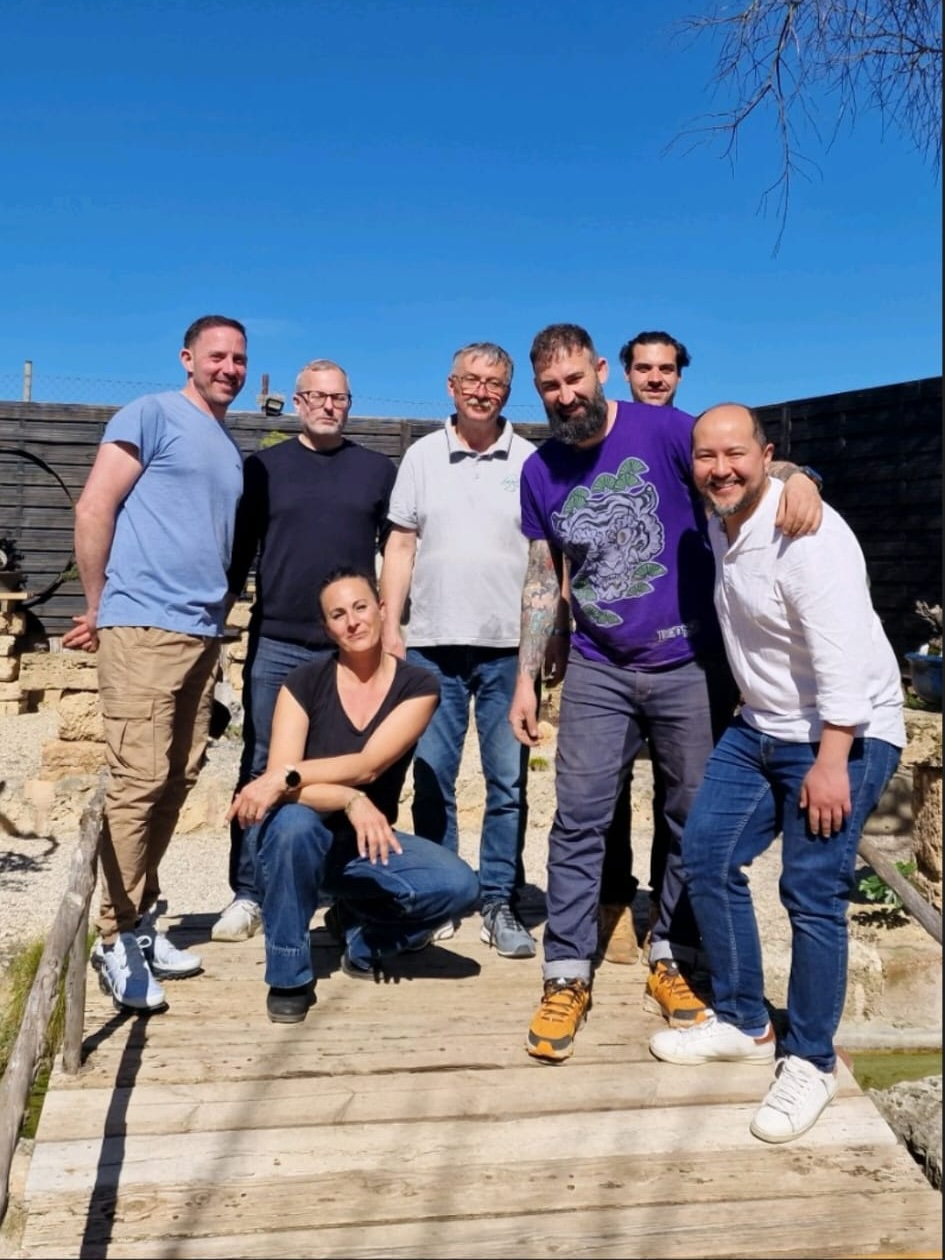
\includegraphics[angle=0,origin=c,width=1.0\textwidth]{2025_05/res/journey_1.jpg}
\end{minipage}\quad
\begin{minipage}[b]{.29\textwidth}
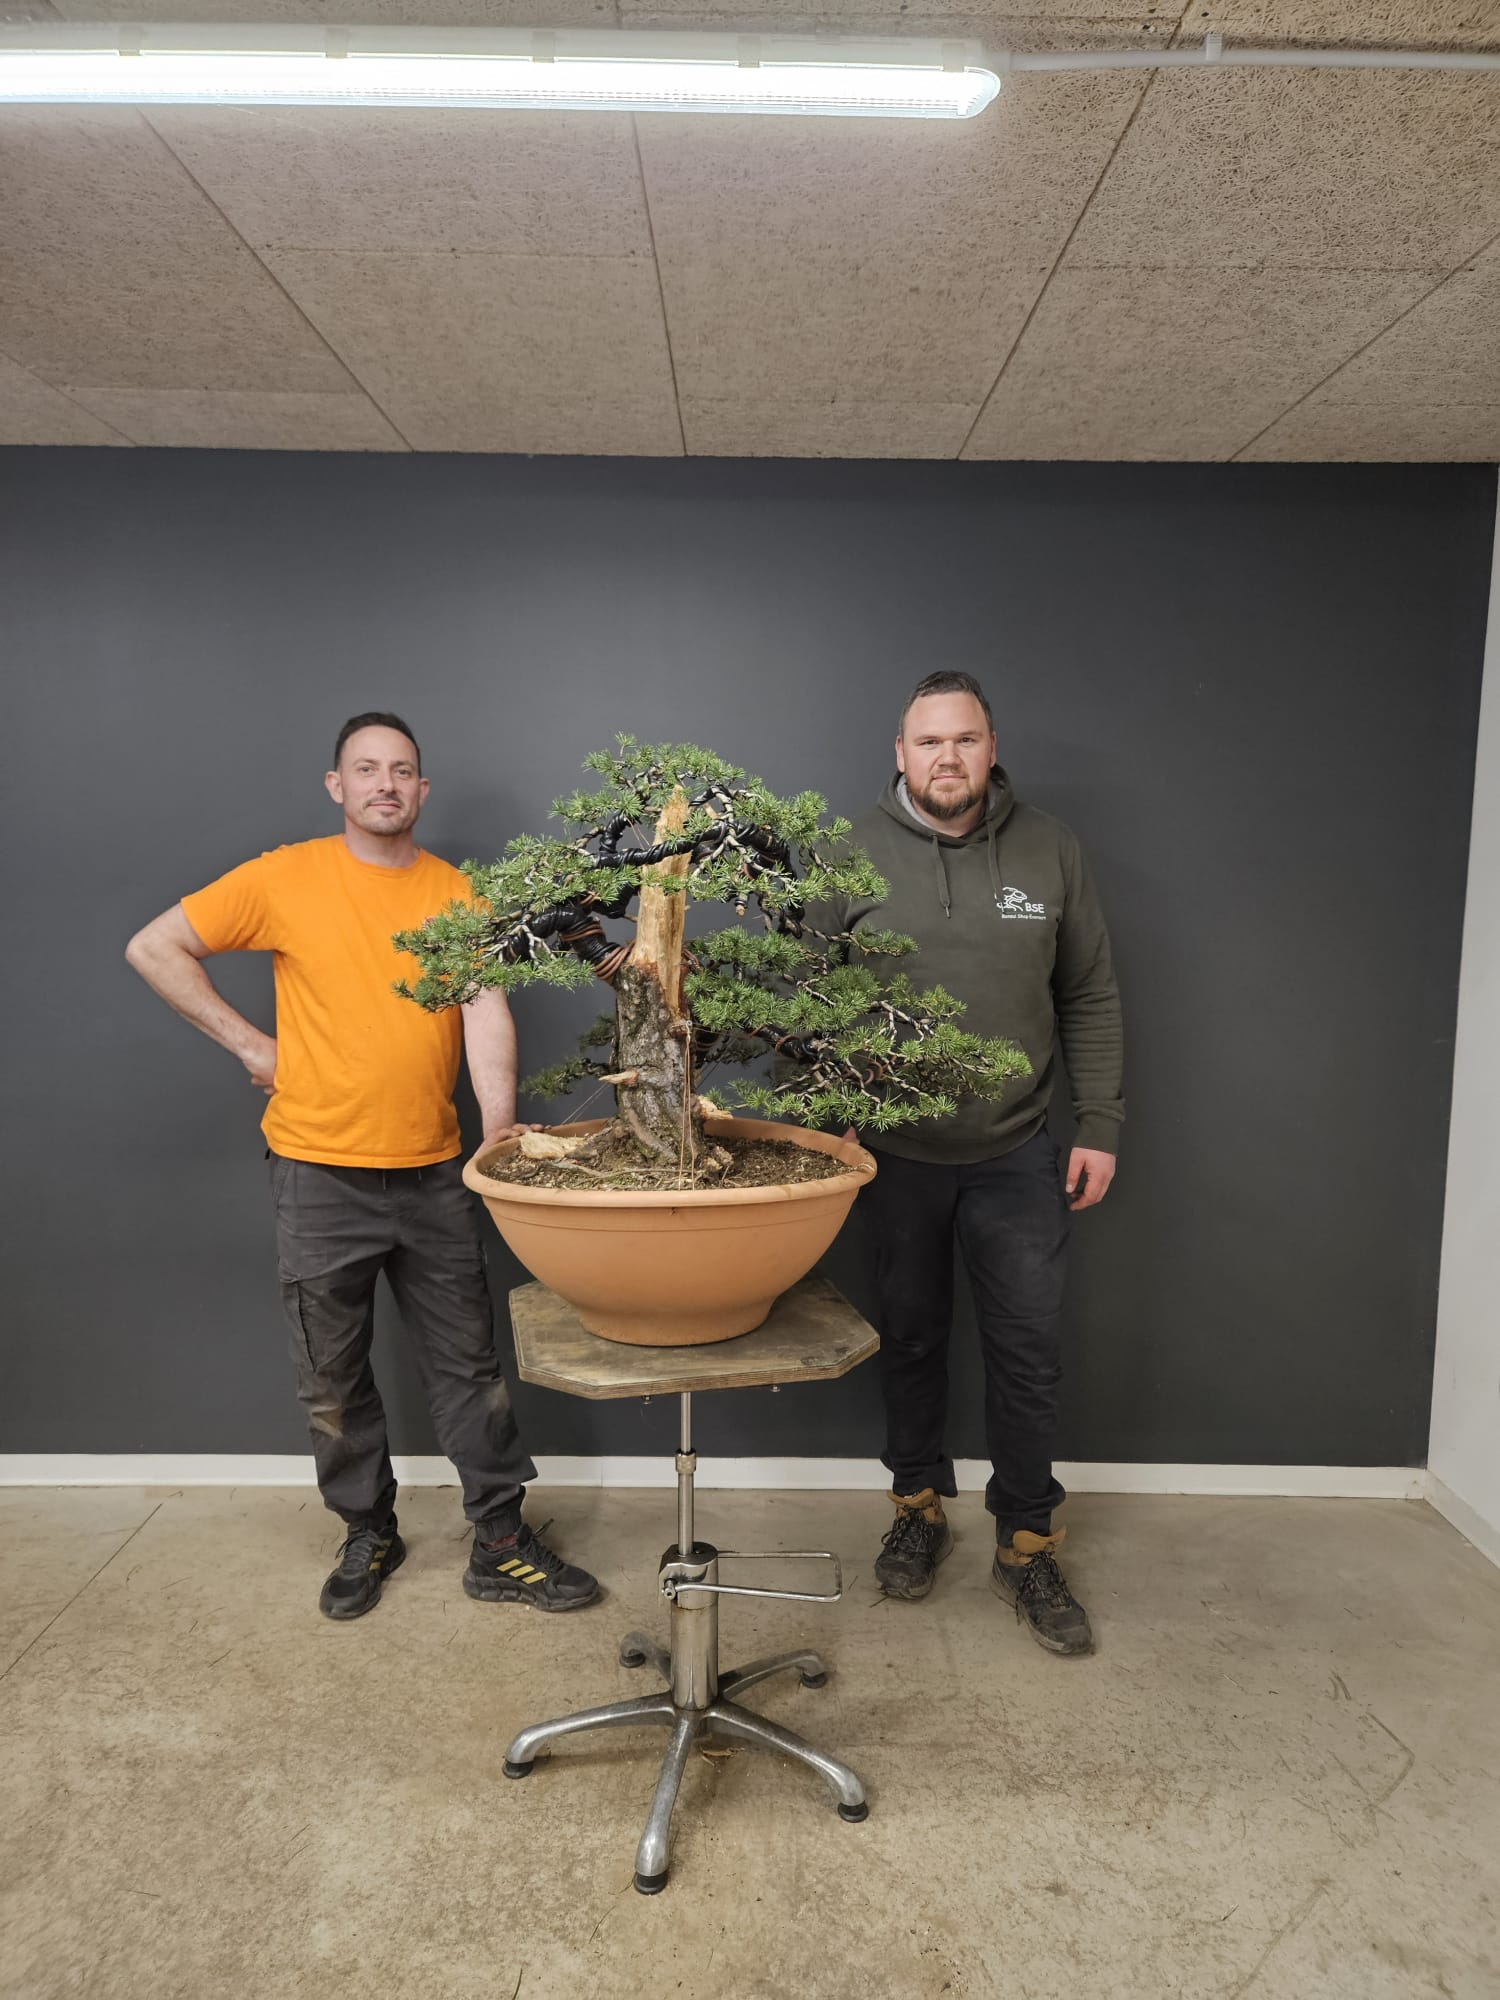
\includegraphics[angle=0,origin=c,width=1.0\textwidth]{2025_05/res/journey_2.jpg}
\end{minipage}\quad
\begin{minipage}[b]{.29\textwidth}
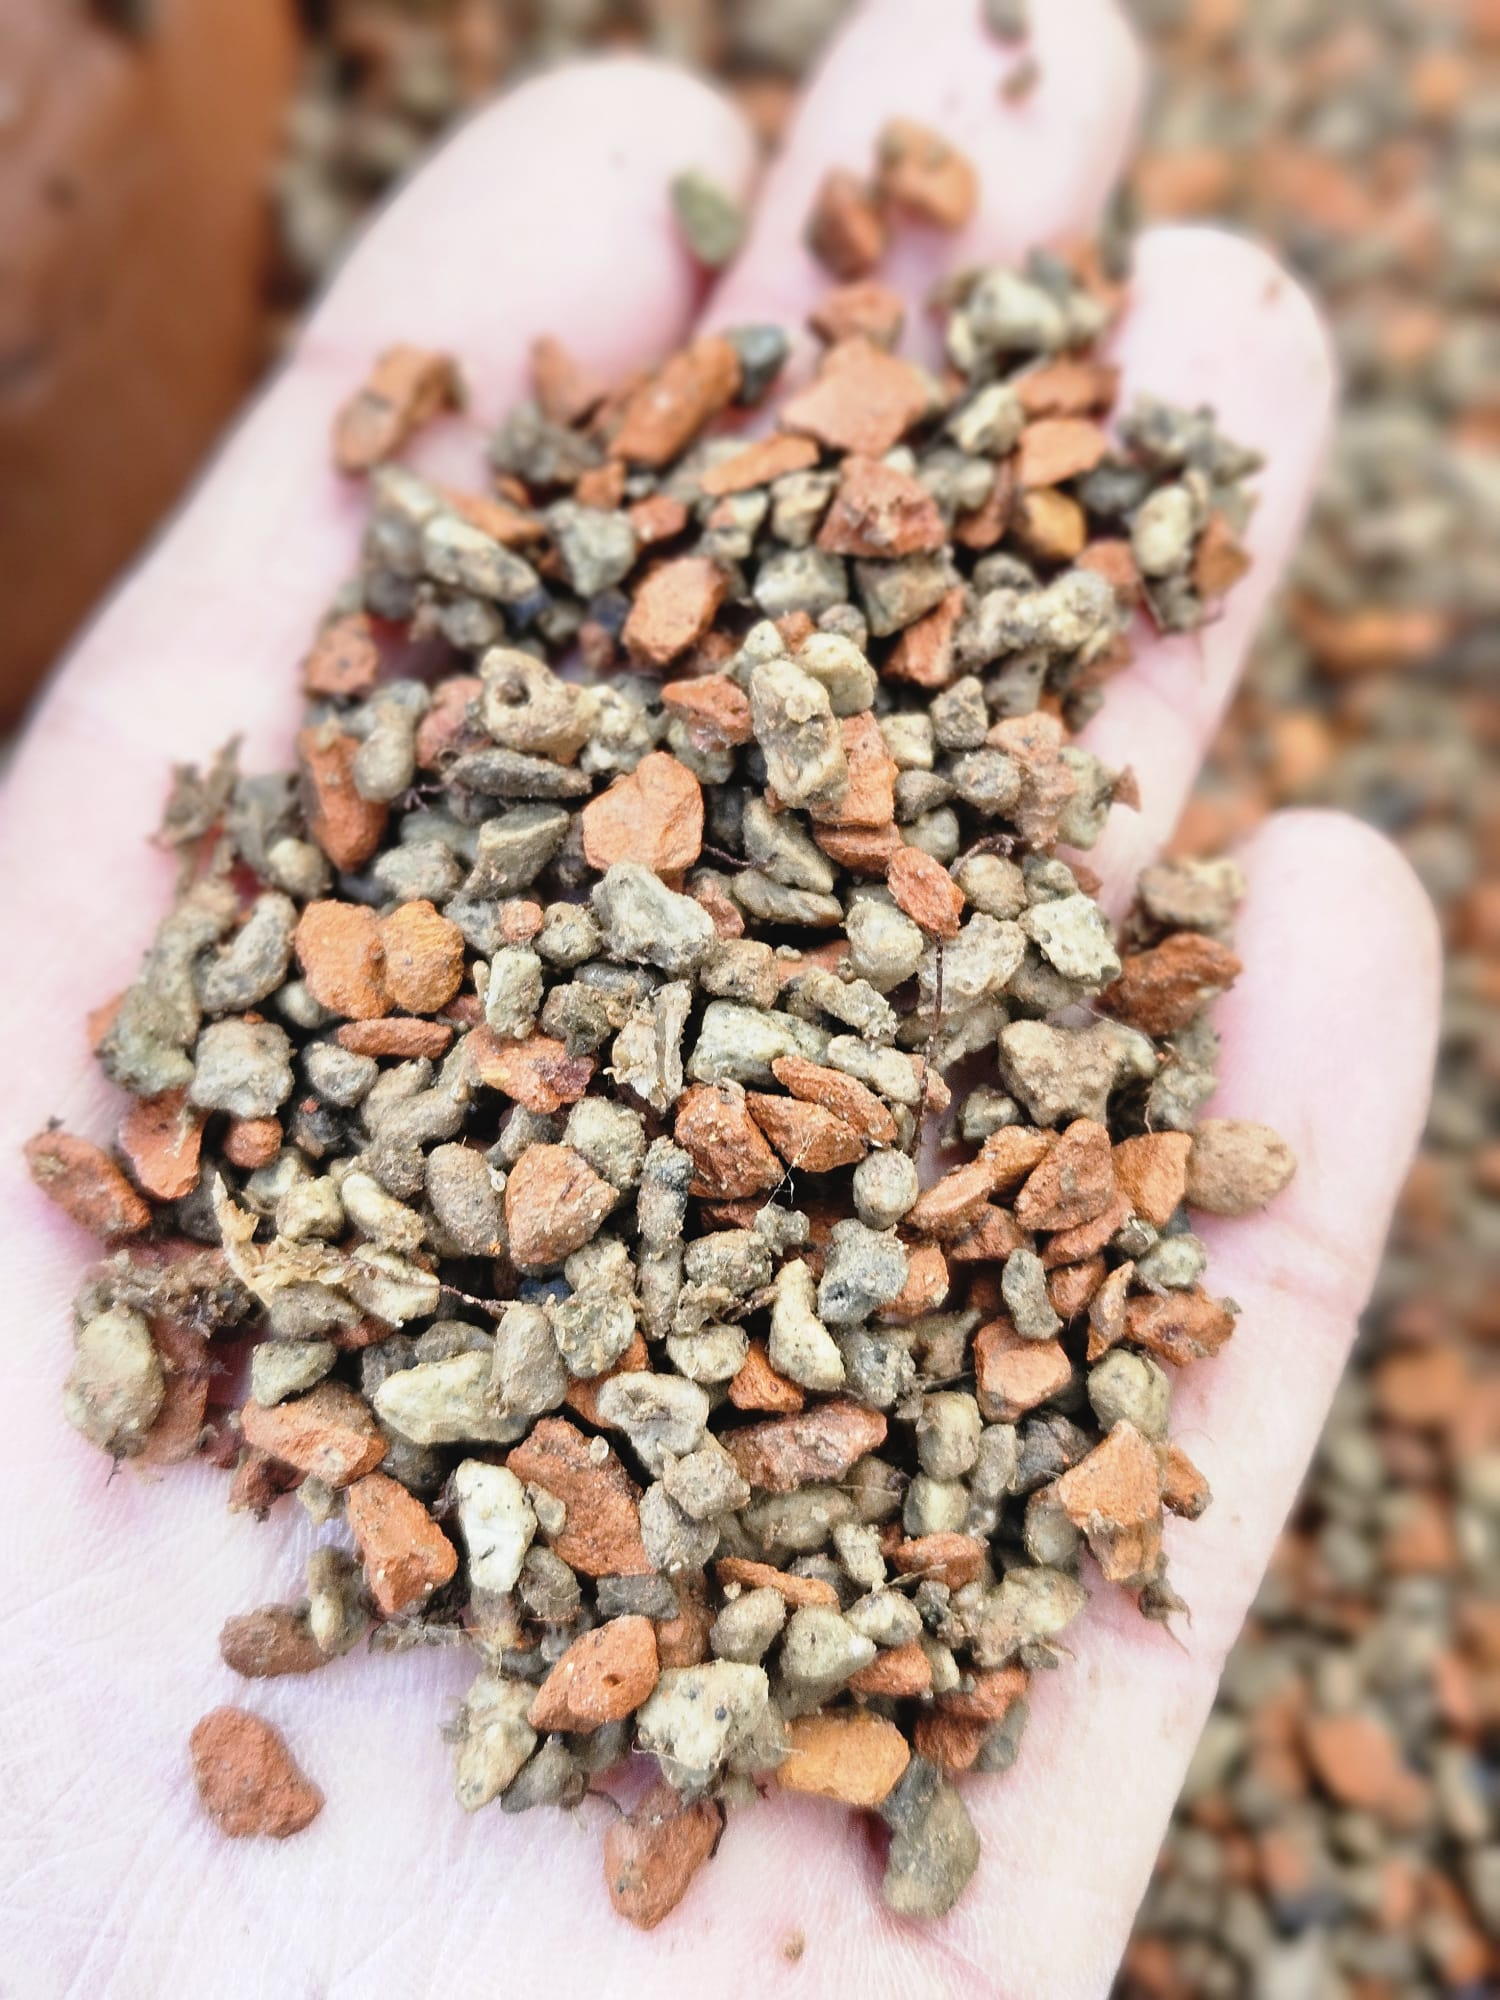
\includegraphics[angle=0,origin=c,width=1.0\textwidth]{2025_05/res/journey_3.jpg}
\end{minipage}\\
\vspace{1em}
\medskip 
\begin{minipage}[b]{.91\textwidth}
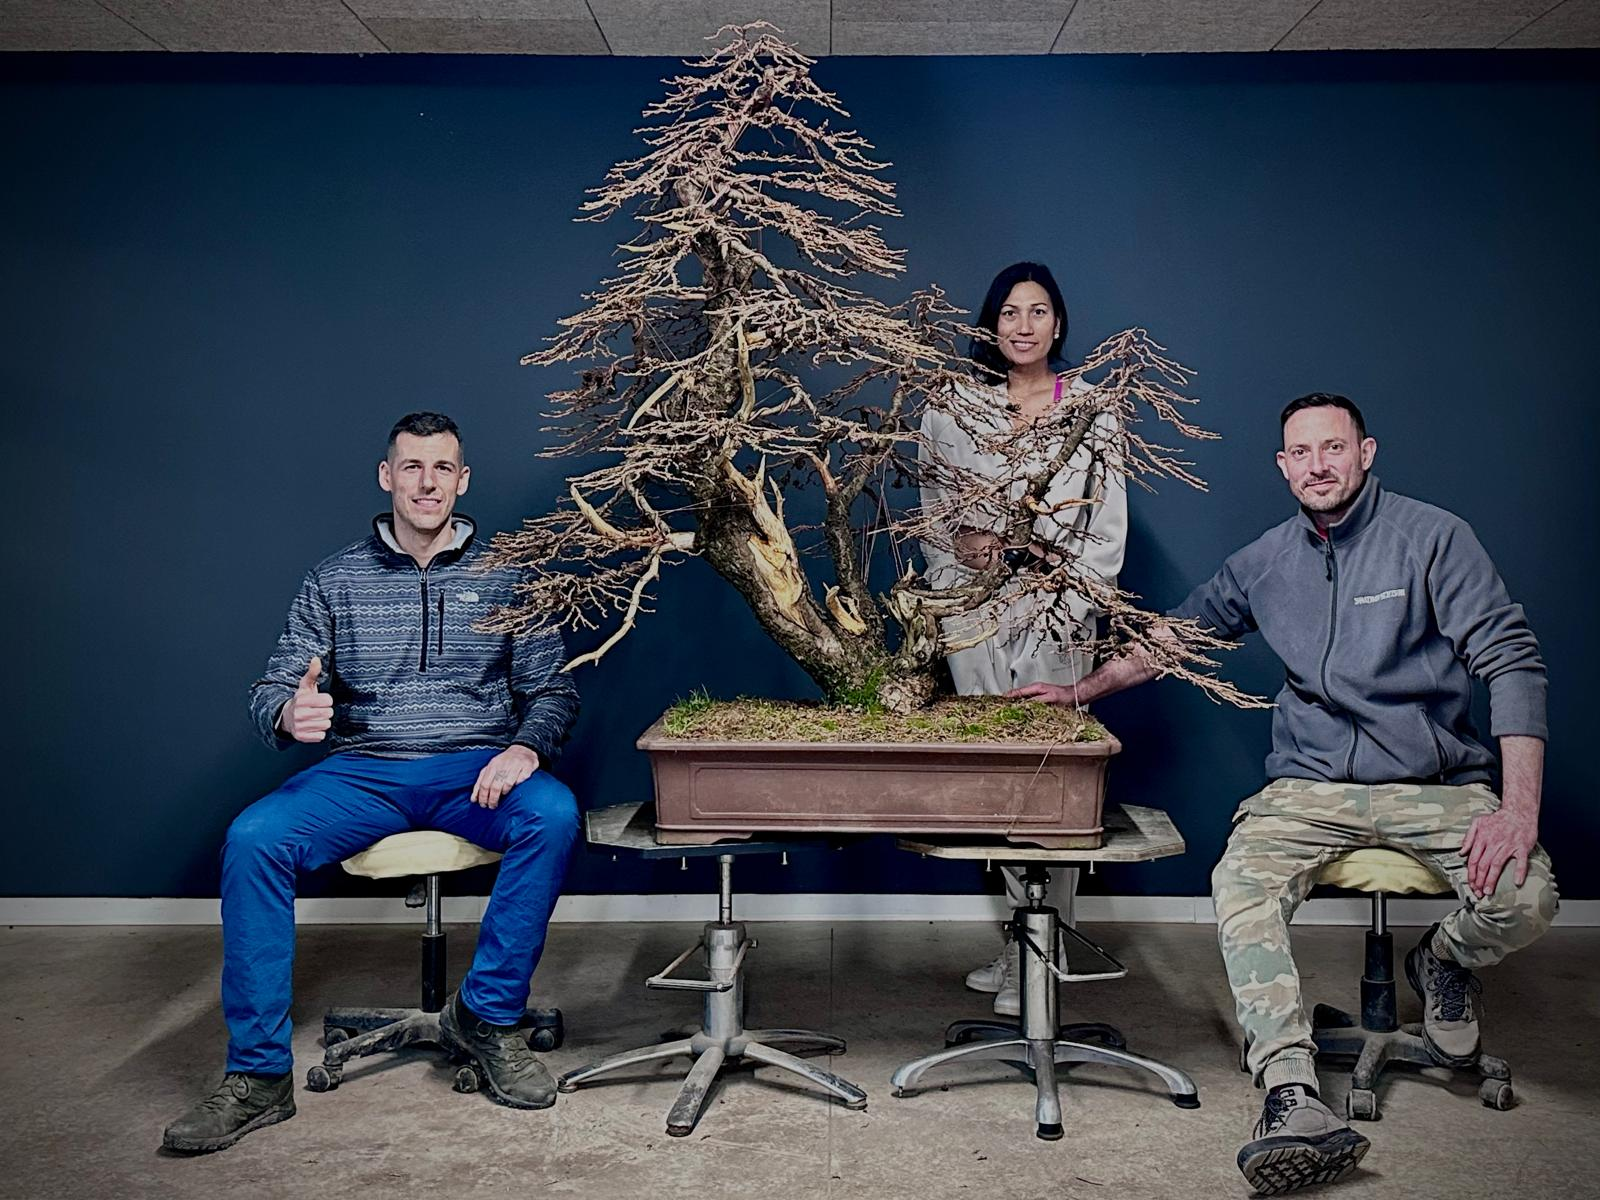
\includegraphics[angle=0,origin=c,width=1.0\textwidth]{2025_05/res/journey_4.jpg}
\end{minipage}
\centerline{\emph{A few highlights from Mark's talk: inspiring visits, thoughtful work, and helpful tips.}}
\end{figure*}
